% Sequence Alignment
%
% A brief, broad introduction to sequence alignment

\subsection{Sequence Alignment}
\begin{frame}
  \frametitle{Alignment Search Space}
  Consider two biological sequences to be aligned$\ldots$
  \begin{itemize}
    \item One sequence on the \textit{x}-axis, the other on the \textit{y}-axis
    \item Each point in space is a pairing of two letters
    \item Ungapped alignments are diagonal lines in the search space, gapped alignments have short ``breaks''
    \item There may be one or more ``optimal'' alignments
  \end{itemize}
  \begin{center}
    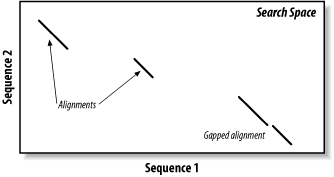
\includegraphics[width=0.4\textwidth]{images/search_space} 
  \end{center}
\end{frame}
    
\begin{frame}
  \frametitle{Global \textit{vs} Local Alignment}
  \begin{itemize}
    \item<1-> Global alignment: sequences are aligned along their entire lengths
    \item<1-> Local alignment: the best subsequence alignment is found
    \item<2-> Consider an alignment of the same gene from two distantly-related eukaryotes, where:
    \begin{itemize}
      \item<2-> Exons are conserved and small in relation to gene locus size
      \item<2-> Introns are not well-conserved but large in relation to gene locus size
    \end{itemize}
    \item<2-> Local alignment will align the conserved exon regions
    \item<2-> Global alignment will align the whole (mostly unrelated) locus
  \end{itemize}
 \end{frame}
